\documentclass{article}
\usepackage[spanish]{babel}
\usepackage[utf8]{inputenc}
\usepackage{graphicx}
\graphicspath{ {./images/} }
\usepackage{hyperref}
\usepackage{subcaption}
\usepackage{geometry} % see geometry.pdf on how to lay out the page. There's lots.
\geometry{a4paper} % or letter or a5paper or ... etc
% \geometry{landscape} % rotated page geometry

% See the ``Article customise'' template for come common customisations


\author{Tomás Bacigalupo , Lucio Pagni}
\date{\today}
\author{Tomas Bacigalupo y Lucio Pagni}
\date{18/07/2020} % delete this line to display the current date

%%% BEGIN DOCUMENT
\begin{document}

% caratula
\begin{titlepage}
\centering
{
\includegraphics[width=1\textwidth]{./images/logoitba.png}\par}
\vspace{1cm}
{\scshape\Large Simulaci\'on de Sistemas \par}
\vspace{3cm}
{\scshape\Huge COVID-19\par}
\vspace{3cm}
{\itshape\Large Trabajo Pr\'actico Final \par}
\vfill
{\Large Autores: \par}
{\Large Tomas Bacigalupo, Lucio Pagni\par}
\vfill
{\Large \today \par}
\end{titlepage}
\clearpage

\listoffigures   % generate list of figures
\clearpage
\listoftables % generate list of tables    
 \clearpage

\tableofcontents
\clearpage

\section{Introducción}
Con el objetivo de estudiar el problema de distanciamiento social en el contexto de la pandemia mundial del covid-19 se trabajo durante la segunda mitad del cuatrimestre en un software de simulación de peatones comprando en un supermercado.Dicho software busca ser más poderoso y configurable que otras versiones comerciales, las cuales usamos como referencia. Nuestro trabajo en el desarrollo fue el de estructurar el proyecto, implementar el main (del cual se desencadenan las llamadas a todos los demás módulos),  y desarrollar el modulo de la caja, cuya tarea es la  de atender clientes y encolarlos en la fila correcta. Por otro lado el trabajo de estructura nos llevo a tomar decisiones como desarrollos de pom.xml con sus respectivas dependencias en cada modulo y como tarea principal se implementaron todos los módulos a travez de un main que permitía mediante un archivo de configuración establecer las variables de la simulación. Y es en este momento donde comienza nuestro trabajo de desarrollo para esta entrega final, donde se mejoraron los tiempos de simulación mediante la mejora de nuestros dos módulos: Main y Caja

\section{Implementación}

\paragraph{}
En esta sección discutiremos todos los aspectos que hacen a la implementación del simulador y la justificación de las decisiones tomadas, tanto de diseño de clases como de diseño de arquitectura.

\subsubsection{La estructura general del proyecto}

En cuanto a la estructura, se optó por una implementación simple de Interfaces e Implementaciones, con el objetivo de programar contra interfaces como se puede ver en la figura \ref{grafico}. 

\paragraph{}
Incialmente la estructura propuesta consistía en una serie de módulos,interconectados y dependientes entre sí mediante una estructura jerárquica. Esta idea inicial no se llevó a cabo por problemas de dependencias cíclicas en esta estructura jerárquica. La estructura de la implementación es conveniente a la hora de definir los testeos unitarios de los métodos implementados y también lo es a la hora de definir archivos de configuración. 

\paragraph{}
En el momento de diagramar el main de la simulación, se hizo un uso intensivo de esta estructura y sus convenciones. Otra ventaja es que nos permite cumplir con los requerimientos impuestos con la cátedra de generar un archivo ejecutable .jar. Una de las bondades de la arquitectura de la implementación es que nos permite obtener dicho ejecutable realizando 'mvn clean package' en la terminal.

\subsubsection{El problema de la configuración}

El simulador debe ser altamente configurable, para esto se implementó una clase aparte llamada ReadConf.java la cual tiene la responsabilidad de leer el archivo de configuración config.properties y servir dichos valores mediante sus variables, las cuales son accesibles desde cualquier clase del proyecto.

\subsubsection{Programación contra interfaces}

\paragraph{}
Como se mencionó anteriormente, es importante poder programar contra interfaces. No solo es muy importante que cada módulo honre correctamente sus interfaces, sino que estas estén bien diseñadas de manera que se abarque el problema de manera completa. Además, se debe tener cuidado de no exponer estado interno de una clase de manera innecesaria. Veremos la justificación de diseño de la interfaz Caja

\paragraph{}
Se expone estado interno de la caja innecesariamente? Por un lado, es verdad que lo mejor sería llamar a cajas.add(agent), o un método del estilo. Sin embargo esto no cubre la complejidad del problema a resolver, esto es porque se deben hacer varias consultas al estado interno de caja antes de insertar definitivamente un agente en la fila. La interfaz de la fila no solo debe darle varios datos a la máquina de estado sino que también debe otorgarlos en instantes distintos del tiempo. Es por eso que la fila provee información que indica a que caja ir y a que posición de cada caja debe ir. Este diseño le permite a la máquina de estados preguntar tantas veces como sea necesario. Además si retornamos unicamente una posición y no el indice de la caja, no estaríamos teniendo en cuanta si su lugar fue ocupado antes por otro agente. En definitiva, los datos expuestos son para que la máquina de estados tenga mas granularidad a la hora de elegir a donde ir y como llegar.

\section{Simulaciones}
Las simulaciones podemos dividirlas en tres grandes grupos. Por un lado se tienen las simulaciones iniciales, en las cuales el módulo caja es solo un boceto. En estas simulaciones se plantea el esquema básico del problema a resolver por el módulo de caja.
Luego se tienen las simulaciones intermedias, estas son, todas las simulaciones que se llevaron a cabo con el simulador integrado. De estas últimas las más importantes son las entregadas para el TP6. Por último se tienen las simulaciones realizadas para evaluar
la mejora en el tiempo de ejecución.

\section{Resultados}
Los resultados discutidos en esta sección hacen referencia a las simulaciones realizadas para evaluar la mejora en el tiempo de ejecución.
Los resultados de las simulaciones antes de las mejoras se pueden ver en la tabla \ref{tablaAntes}.
Los resultados de las simulaciones despue\'es de las mejoras se pueden ver en la tabla \ref{tablaDespues}.

\section{Concluciones}
Observando los resultados podemos concluir que las mejoras realizadas en el código lograron el objetivo de disminuir el tiempo de ejecución.

\section{Apéndice}
texto

\clearpage
\section{Figuras}
\begin{figure}[h]
\begin{center}
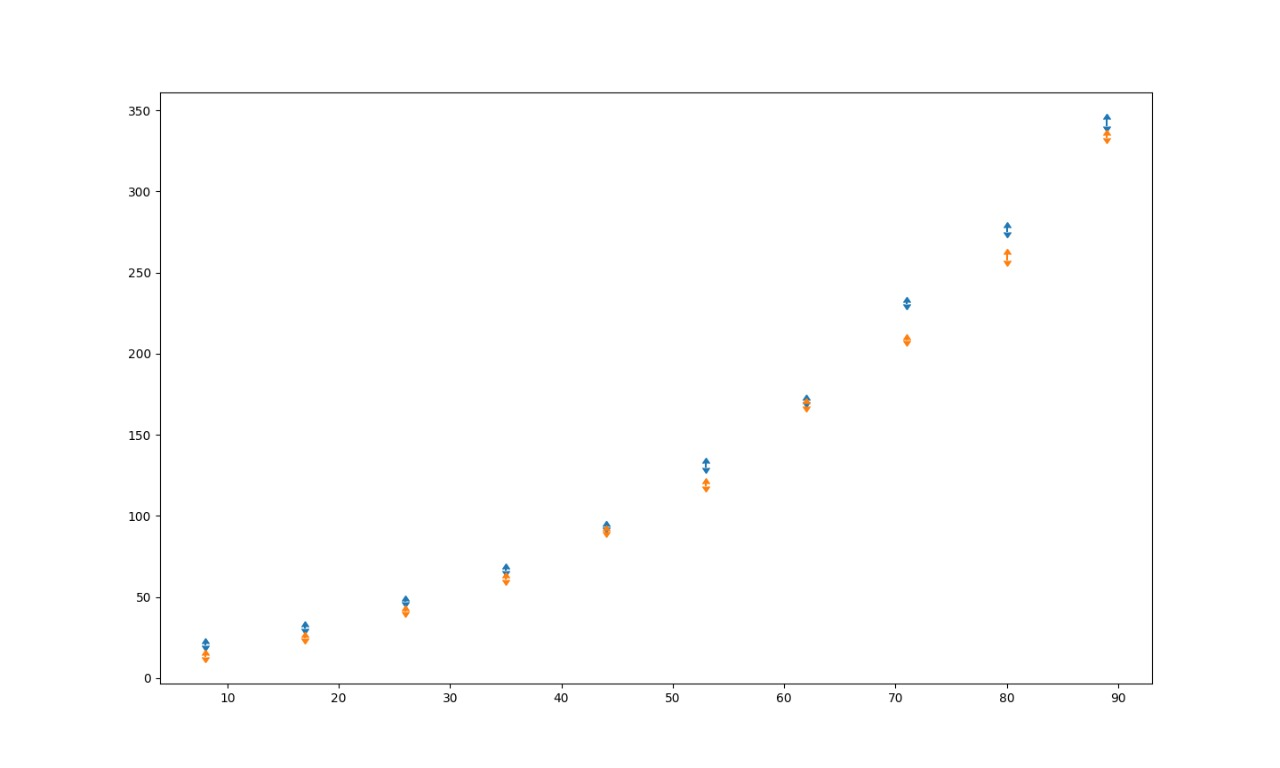
\includegraphics[width=4in]{./images/inputVsOutput.jpeg}
\caption{Ejemplo aca va la descripcion }
\label{grafico}
\end{center}
\end{figure}
\clearpage

\end{document}